\chapter{FPGA-based Implementation of The DNA Recombination Algorithm\label{chapter:FPGA}}
In this Chapter, we study the implementation of $V(D)J$ recombination process on FPGA using the n-necleotide level parallelism that was used in the GPU-based implementation in Section \ref{sec:N-level}. As we converge to a final hardware architecture, we provide a detailed explanation for each unit individually. We explain the experimental results for the n-level FPGA-based implementation of $V(D)J$ recombination process in Section \ref{sec:simNlevel}. Based on the simulation results, we explain the draw back of n-level paralleization method for FPGA-based implementation of the recombination process in Section \ref{sec:drawbackNlevel}. As a result, we proposed the VJ level parallelization approach for the FPGA-based implementation to overcome the draw back of n-level approach in Section \ref{sec:VJ level}. We describe the structure of each unit of the final hardware architecture for the VJ method. Finally, we describe the simulation results for the new parallelization approach in Section \ref{sec:simVJlevel}. 



\section{Hardware Implementation of N Level Parallelization }\label{sec:N-level}

The goal for the hardware implementation of DNA recombination process is to accelerate the generation of all possible TCR sequences with any given $V$, $D$ and $J$ gene sequences and count the number of times each sequence can be generated artificially. As we converge to a final hardware architecture for this process we need to determine the level of parallelism and granularity of the processing elements for generating \emph{in silico} sequences, orchestrate the data transfers between the memory  and computation units, and balance the trade-off between throughput and resource usage. In this section, we first  describe the parallelization strategy and then explain the structure of each unit that is used to implement the $V(D)J$ recombination algorithm.
%individually in Section \ref{subsec:Parallel}. 
%Second, we provide a detailed explanation for the structure of input data set in section \ref{subsec:dataset}. 
%Then, we explain the structure of each unit individually in Subsections \ref{subsec:processing unit} - \ref{AGU}. 

Fig \ref{fig:BIG-Picture_NLevel} shows the proposed architecture for the hardware implementation of the recombination process, which consists of three units, address generator unit (AGU), memory bank unit, and  processing unit. The processing unit (PU) consists of processing element (PE), n-sequence initiator, and \emph{in vivo} address generator units. The PE consists of a number of parallel computation units (CUs), which is formed of concatenation and comparison units.   

The PU generates the number of times  each \emph{in vivo} sequence can be generated artificially in cooperation with the memory bank unit and corresponds to the inner most three loops in Algorithm \ref{Algorithm:2}. The n-sequence initiator provides the legitimate n-nucleotide length and reference n-nucleotide sequence for each CU based on the length of each input  $V$, $D$ and $J$ gene sequences. Each CU  generates a unique  n-nucleotide sequence, forms all possible  \emph{in silico} sequences based on  the input $V$, $D$ and $J$ gene sequences,  and searches those generated sequences in the \emph{in vivo} memory bank. The \emph{in vivo} address generator unit allows reading the \emph{in vivo} sequences and their counter values for each CU, and updates the counter value when a match is found by a CU. The AGU is corresponds to the outer most three for loops in Algorithm \ref{Algorithm:2} in order to generate the indexes for accessing the $V$, $D$, $J$ sequences.  The memory bank unit is compromised of four sub-memory banks for maintaining input and output data sets. 



\begin{figure}[t!]
\begin{center}
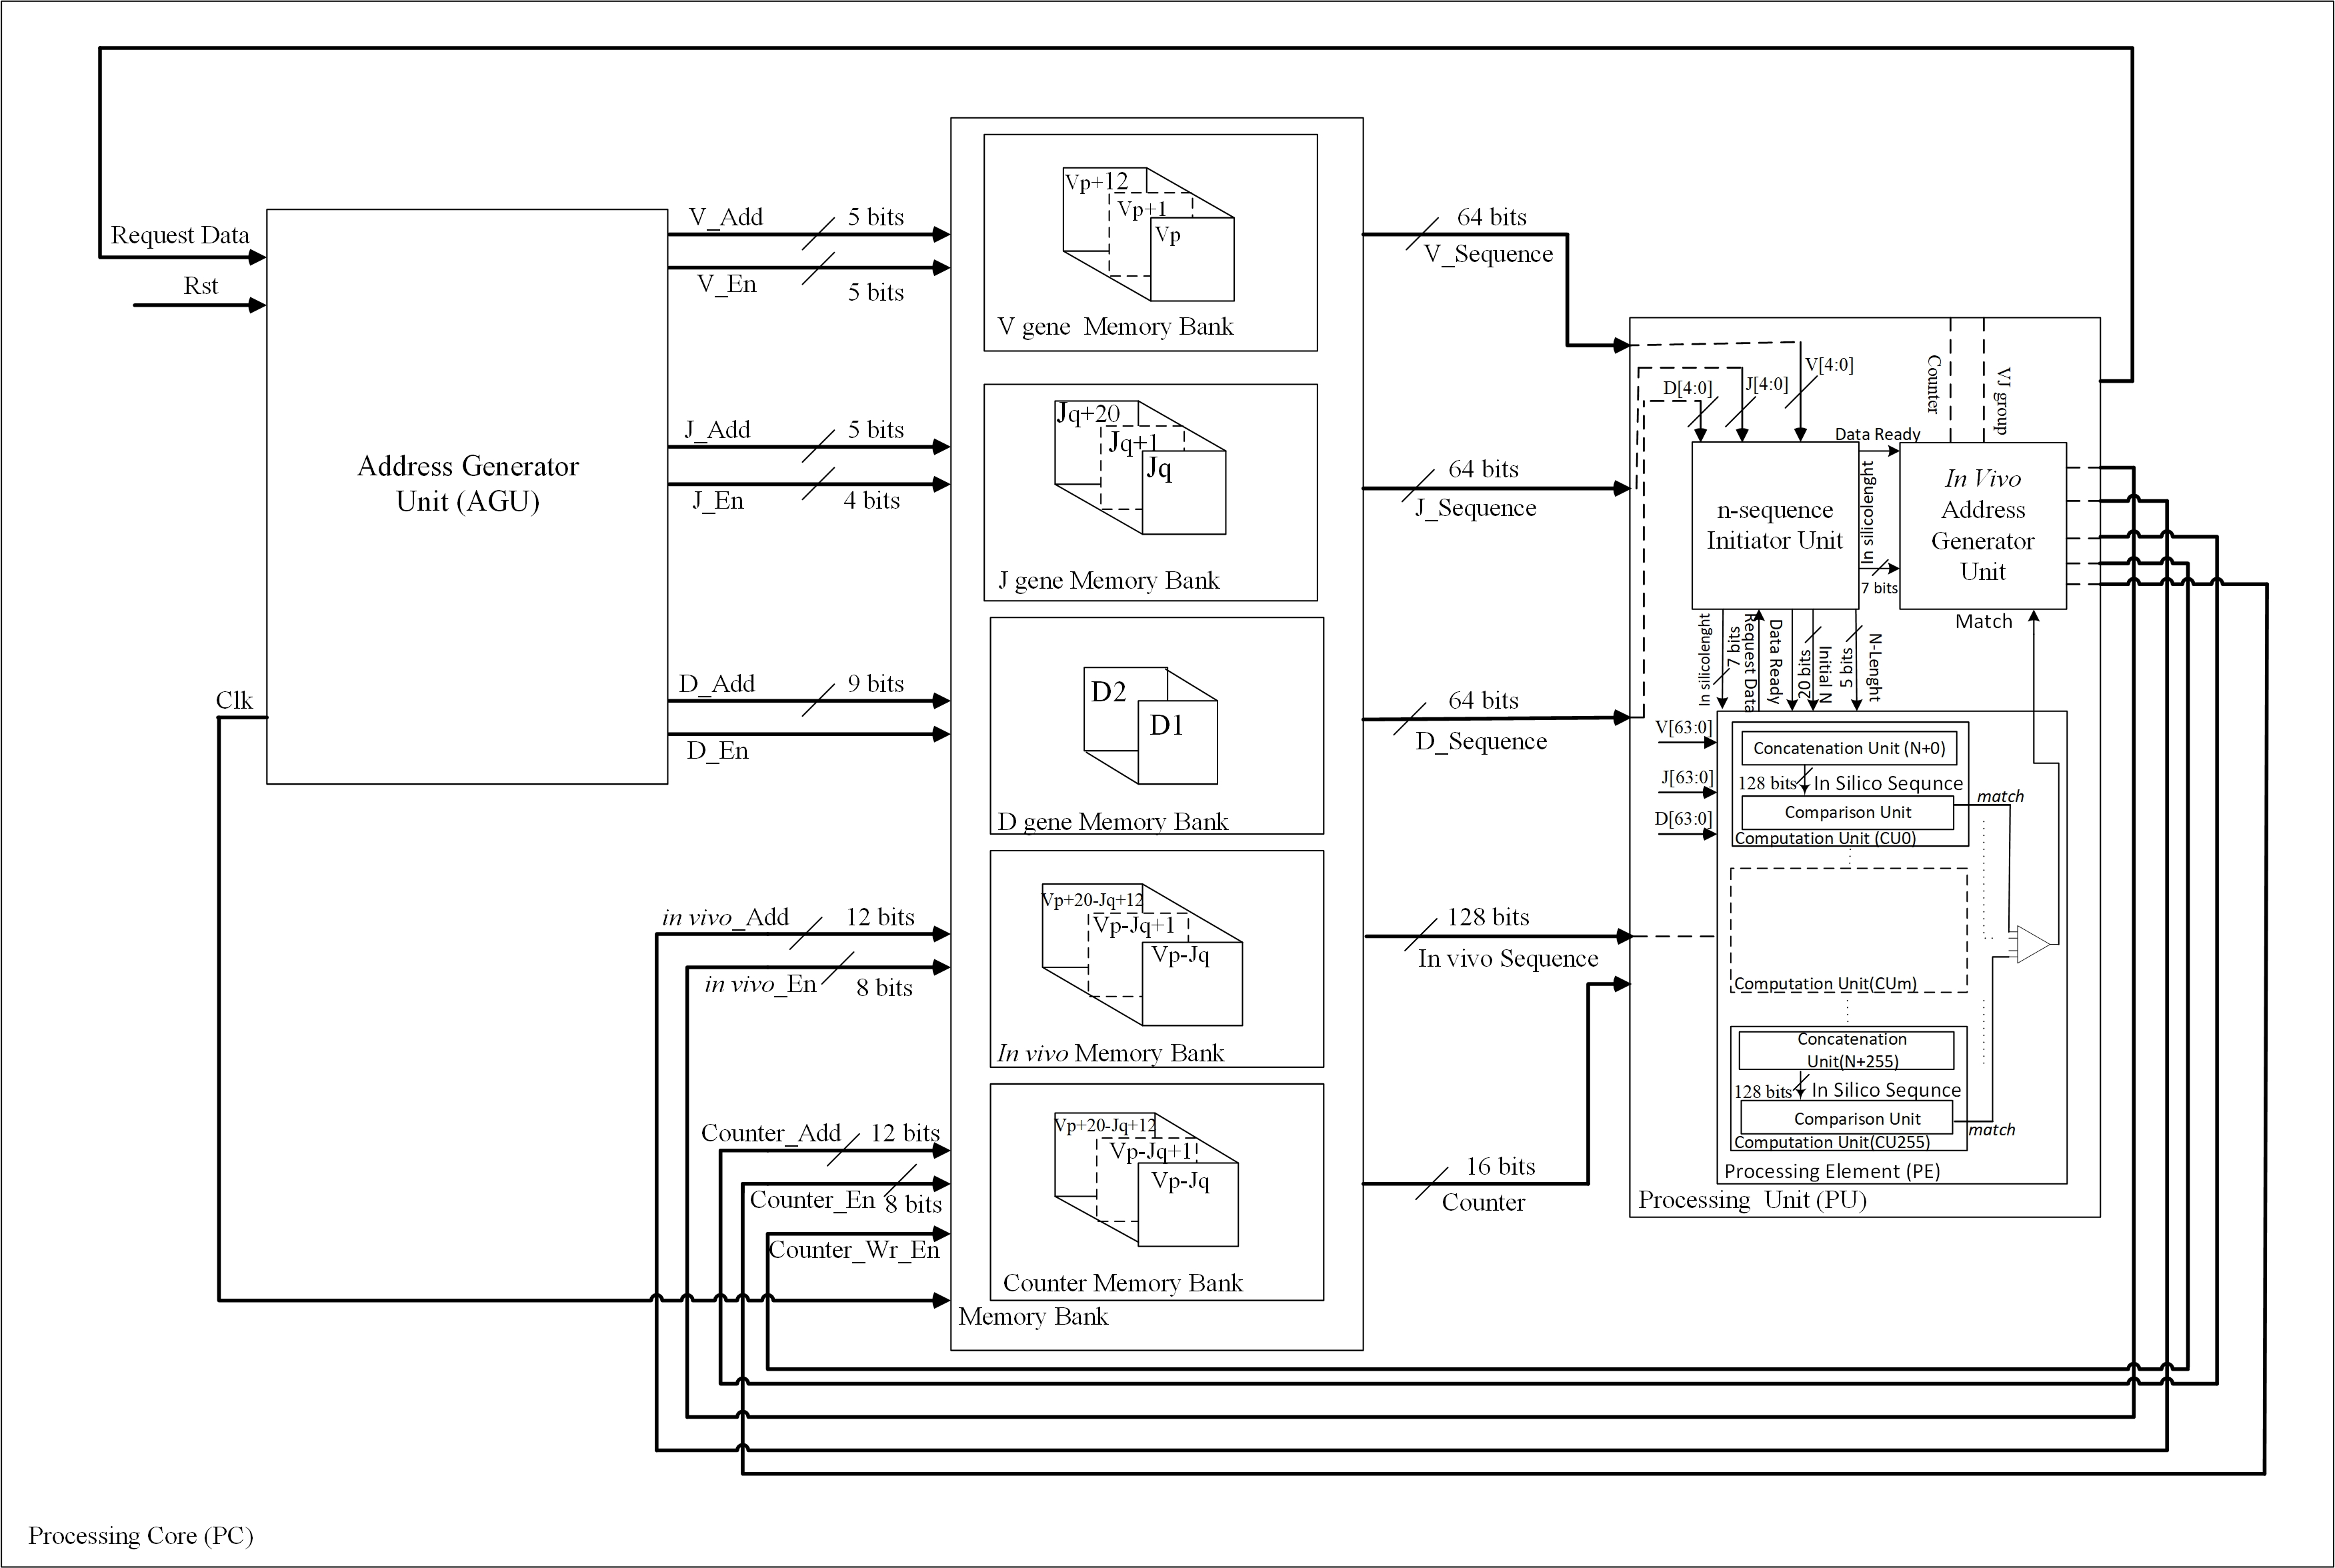
\includegraphics[clip,width=1\columnwidth]{Fig/BIG-Picture_NLevel.jpg}
\caption{The hardware implementation of $V(D)J$ recombination process using the N-level parallelization approach.}
\label{fig:BIG-Picture_NLevel}
\end{center}
\end{figure}

\subsection{N Level Parallelization Strategy}\label{subsec:Parallel}

In this section, we present a series of experimental analysis to answer the following four questions that will help us determine the degree of parallelism ($D_{p}$) to realize in the final architecture:

1) What is the efficient parallelization strategy that will minimize the execution time, 
2) How does the workload partitioning strategy across the CUs affect the performance based on the resource constraints imposed by the target FPGA,
3) What is the correlation of the $D_p$ with the resource utilization and the critical path delay, and
4) How does the $D_p$ affect the throughput?

As mentioned in Chapter \ref{sec:DNA}, all possible forms of n-nucleotide sequences are involved in the recombination process. The length of n-nucleotide ($N_{length}$) can be between zero to ten and the n-nucleotide sequence can be placed on either side of $D$ sequence. Table \ref{tab:1} shows the total number of unique n-nucleotide sequences based on the $N_{length}$ along with the total number of possible combinations of $n_{1}$D$n_{2}$ with a given $D$ sequence given that $D$ gene can partition the n-nucleotide of  size $N_{length}$ at any position generating $N_{length}+1$ such partitioning opportunities. Therefore, if the length of $D$ sequence is greater than zero then, the total possible combinations is equal to $4^{ N_{length}} \times (N_{length}+1)$.

The computation requirement is the same for generating  the \emph{in silico} sequences based on each of the $4^{ N_{length}}$ unique n-nucleotide sequences. This creates an opportunity to parallelize at n-nucleotide level and achieve a balanced workload distribution across the computation units. This was the parallelization approach taken in our GPU-based implementation to achieve a balance workload across the threads and thread blocks of the GPU.  
Consider the case of $N_{length}$ of ten, which generates over one million unique sequences. Hardware implementation at a scale of million CUs is not feasible due to  the resource constraints. Therefore a partial parallelization is needed and the resource demand for a single CU helps us determine the amount of unrolling we can apply to the loop with index four in Algorithm \ref{Algorithm:2} and derive the number of CUs we can instantiate on the target FPGA. This number will also help us determine the structure of the n-sequence initiator and PU. Therefore, in order to answer the second question, we implement a single CU, that is composed of concatenation and comparison units on the the Virtex-7 XC7VX485T FPGA. We will describe the details of the PU structure in section \ref{subsec:processing unit}. As shown in table \ref{tab:2}, the "Slice LUTs" is the determining factor and we can fit up to 256 CUs leaving 15\% of the resources for the AGU state machine, $n-$sequence initiator unit, \emph{in vivo} address generator and glue logic. 

In order to answer the third question, we implement the proposed architecture for different $D_p$ and plot the resource utilization trend as shown in Fig. \ref{fig:ResourceUtil}. As we increase the $D_p$, the resource utilization increases linearly. We show the critical path delay with respect to changes in $D_p$  in Fig. \ref{fig:CriticalPath} to answer the third question. As shown, the critical path delay slightly increases as the $D_p$ increase. 

In order to answer the last question, we first need to define the throughput. The throughput is defined as the total number of comparisons per second. Since, we have the same number of comparison units as the $D_P$, the throughput increases linearly.

Based on the above analysis, we set the $D_P$ equal to 256 and the final architecture based on our n-nucleotide level parallelization strategy is shown in Fig. \ref{fig:BIG-Picture_NLevel}. In the following sections, we explain the structure of each unit within the processing core (PC) in detail.

\begin{table}[t!]
\caption{The total number of unique n-nucleotide sequences and total number of possible combinations of  $n_1$D$n_2$ with a given $D$ sequence based on the length of n-nucleotide.}
\begin{center}
\begin{tabular}{ |c|c|c| }
  \hline
    \textbf{\textit{$N_{length}$}} & \textbf{\textit{Total number of unique}} & \textbf{\textit{Total number of possible}}\\
    ~ &  \textbf{\textit{$n-nucleotide$ sequences}} & \textbf{\textit{combinations of $n_1$D$n_2$}}\\
    ~&~& \textbf{\textit{with a given D }}\\ \hline	
    0 & 1  	& 4	\\	\hline
    1 & 4 	& 8	\\	\hline
   	2 & 16 	& 48\\	\hline
    3 & 64 	& 256	\\	\hline
    4 & 256 & 1280	\\	\hline
    5 & 1024 &6144 	\\	\hline
    6 & 4096 & 28672	\\	\hline
   	7 & 16384 &131072 	\\	\hline
    8 & 65536 &	589824\\	\hline
    9 & 262144  &2621440 \\	\hline
    10 & 1048576 & 11534336\\
  \hline
\end{tabular}

  \label{tab:1}
\end{center}
\end{table}

\begin{table}[t!]
\caption{Resource Utilization for a single CU}
\begin{center}
\begin{tabular}{ |c|c| }
  \hline
    Slice LUTs (303600) & 977 \\	\hline
    Slice Registers (607200) & 509\\	\hline
    Slice (75900) & 275	\\hline
    LUT as Logic (303600)& 977\\	\hline
    LUT Flip Flop Pairs (303600) & 272\\
  \hline
\end{tabular}

  \label{tab:2}
\end{center}
\end{table}

\begin{figure}[t!]
\begin{center}
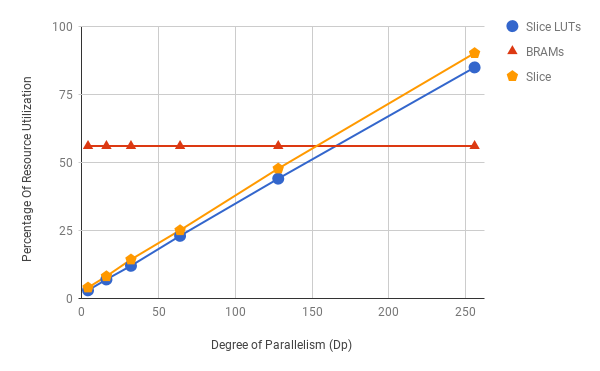
\includegraphics[clip,width=1\linewidth]{Fig/Chart.png}
\caption{The resource utilization of the N-level architecture for different values of the $D_P$. }
\label{fig:ResourceUtil}
\end{center}
\end{figure}



\begin{figure}[t!]
\begin{center}
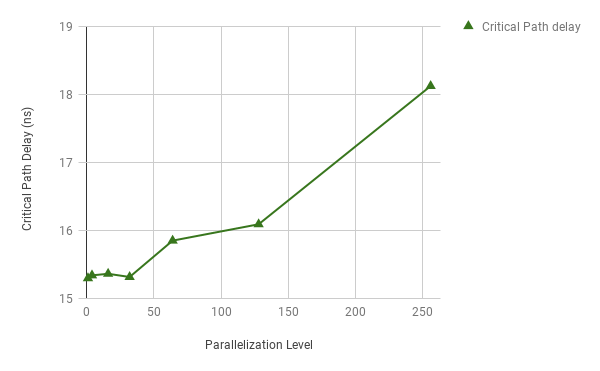
\includegraphics[clip,width=1\linewidth]{Fig/CriticalPathDelay_ParallelizationLevel.png}
\caption{The critical path delay of the N-level architecture for different values of the $D_P$. }
\label{fig:CriticalPath}
\end{center}
\end{figure}
%\subsection{Input Data Sets}\label{subsec:dataset}
%%%%%%%%%%%%%%%%%%%%%%%%%%%
%The input data sets consist of $V$, $D$, $J$ and \emph{in vivo} genes. In C57BL/6 mice, there are 20 basic $V \beta$ genes, 2 $D \beta$ genes and 12 basic $J \beta$ genes. However, all possible patterns such as chewback and palindromic forms for each of the functional $V$, $D$ and $J$ gene sequences need to participate in the recombination process for modeling the TCR repertoire as illustrated in  Fig\ref{fig:VDJ}. 
%For example, the first basic $V$ gene has a length of 14. For the $V$ gene, up to four genes can be appended to the right end of the $V$ gene from its mirror strand (step one, indicated as +4, +3, +2, +1), therefore the actual length of this gene can be up to 18. This would result with 18 different sequences based on the chewback process (step two). $D$ and $J$ gene data sets go through similar process as explained in section \ref{subsec:Bio}, therefore each $V$, $D$ and $J$ gene data set consists of several forms of sequences with different lengths. In C57BL/6 mice, the \emph{in vivo} data set involves 101822 sequences, which are grouped based on the specific $VJ$ pair used to generate that sequence. There is no other recombination path for an \emph{in vivo} sequence other than the specific $VJ$ pair, which generates that specific sequence. This is a key feature that we will exploit to reduce a search space for the \emph{in vivo} address generator unit and reduce the execution time . There are 240 such pairs since we have 20 basic $V$ genes and 12 basic $J$ genes in mice.



%%%%%%%%%%%%%%%%%%%%%%%%%%%%%%%%%%%%%%%
\subsection{Processing Unit}\label{subsec:processing unit}
%%%%%%%%%%%%%%%%%%%%%%%%%%%%%%%%%%%%%%

As illustrated in Algorithm \ref{Algorithm:2}, modeling the TCRs repertoire involves six nested for loops. We map the inner most three for loops with index 4-6 to the PU to iterate through all possible forms of n-nucleotide additions, create \emph{in silico} sequences, and search for a match of the \emph{in silico} sequence within the \emph{in vivo} data set. We describe the structure of the PU composed of the PE, $n$-sequence initiator, and \emph{in vivo} address generator units in the following subsections.

The inputs to the PU are the $V$, $D$, $J$, and \emph{in vivo} sequences received from their respective memory bank units, the counter received from the conuter memory bank unit, and the VJ group ($group_{id}$) from the AGU. The addresses for these three sequences are determined by the AGU, which will be discussed later. We set the bitwidth for each sequence to 64 as shown in Fig. \ref{fig:BIG-Picture_NLevel}. In C57BL/6 mice data set, the maximum length of the  $V$, $J$ and $D$ gene sequences is 26 characters. We assign two bits to represent each of the four types of nucleotide bases (A, G, C, and T). We reserve five bits to keep track of the length of each sequence. The n-sequence initiator unit will rely on this length information for selecting valid length for the n-nucleotide sequence. In addition, the concatenation unit depends on the length information for generating the \emph{in silico} sequence. As explained earlier in Chapter \ref{sec:DNA}, the $D$ gene goes through chewback process on its both ends. Based on the C57BL/6 mice data set, there are maximum of 22 different paths to generate $D$ sequences. We reserve five bits to represent each path, which we refer to as $D_{Path}$. The \emph{in vivo} address generator unit will require this information for counter update, which will be discussed later. Therefore, in total we need to form a 62 bit package as an input to the PU, however we set the package size as 64 leaving 2-bit  for debugging purpose to set as used or not used.  
 
%%%%%%%%%%%%%%%%%%%%%%%%%%%%%%%%%%%%%%%
\subsection{n-sequence Initiator Unit }\label{subsec:nsequence}
%%%%%%%%%%%%%%%%%%%%%%%%%%%%%%%%%%%%%%
The input to the n-sequence initiator unit are the length of $V$, $D$, and $J$ gene sequences received from their respective memory bank units, the $Request Data$ signal received from the PE. The outputs of this unit are the $Data Ready$, $N_{length}$, length of \emph{in silico} sequence ($sequence_{length}$), and the reference n-nucleotide sequence ($Initial_N$) for the CUs, and $Data Ready$ and $sequence_{length}$ for the \emph{in vivo} address generator unit. We set the bitwidth of $N_{length}$ and $Initial_N$ to five and 20 respectively, as the maximum length of n-nucelotide is 20 bits (ten characters). Also, we set the bitwidth of $sequence_{length}$ to seven as the maximum value for $sequence_{length}$ is 120 bits (60 characters).  

The n-sequence initiator unit implements the for loop indexed  as four in the Algorithm \ref{Algorithm:2}. This loop iterates through n-nucleotide of length zero through ten and generates all possible sequences for that length. We can extend the for loop with index of four into three sub-for loops as shown in Algorithm \ref{Algorithm:1}. 

The first for loop iterates through all possible n-nucleotide sequences of $N_{length}$ between zero and ten. However, all possible n-nucleotide sequences for each length will not result with valid \emph{in silico} sequence based on the given $V$, $D$ and $J$ gene sequences as the $sequence_{length}$ must be within the range of six to sixty characters and divisible by three. Therefore, primary functionality of the n-sequence initiator unit is selecting the legitimate $N_{length}$ and proceed to the next loop. The second for loop iterates through all possible unique n-nucleotide sequences for the selected $N_{length}$. Table \ref{tab:1} shows the total number possible unique n-nucleotide sequences with different length. 

Rather than having this unit generate a n-nucleotide sequence for each CU, and send all possible combinations in rounds each with 256 sequences (as there are 256 parallel CUs), we send only $Initial_N$ as a reference starting address to all CUs and have each CU calculate its unique n-nucleotide sequence using $Initial_N + CU_{id}$, expression where $CU_{id}$ is the index of CU. This allows us to reduce the amount of data transfer to the CUs and wiring requirement on the implementation. After each round, the $Initial_N$ is incremented by 256 to complete all the rounds needed for that specific $N_{length}$, which is  $4^{N_{length}}/256$. The third for loop iterates through all possible combinations for the length of  $n_1$ and $n_2$ sequences to cover all forms of $n_1$D$n_2$ sequence. 

\begin{algorithm}[t]
 
\nl \For{$i = 0$ to 10}{
		\emph{$N_{length}$} = i;
		
		$sequence_{length}$ = $V_{len}$+ $J_{len}$ + $D_{len}$ + $N_{length}$;
		
		\If{$(6<=sequence_{length}<=60)~\&~(sequence_{length} \% 3 == 0)$ }{
			
			\nl     \For{$k = 0$ to $4^i$}{
		
		$Initial_N$ = $k$;
		
		\nl     \For{$j = i$ to 0}{

		$len_{n_{1}}$ = j;
		
		$len_{n_{2}}$ = i-j;
		}
		$k$ = $k$ + $D_P$;
  
}
		}
		

}
 \caption{Pseudo code for expanding the for loop with index of four in Algorithm \ref{Algorithm:2}. }
\label{Algorithm:1}
%vspace{-.5em}
\end{algorithm}


%%%%%%%%%%%%%%%%%%%%%%%%%%%%%%%%%%%%%%%
\subsection{In vivo Address Generator Unit }\label{subsec:InVivoAGU}
%%%%%%%%%%%%%%%%%%%%%%%%%%%%%%%%%%%%%%
The inputs for the \emph{in vivo} address generator unit are the $sequence_{length}$ and $Data Ready$ from the n-sequence initiator, the $group_{id}$ from the AGU, the $Match$ signal indicates that there is a match between \emph{in vivo} and \emph{in silico} sequences, from the $PE$, and the 16-bit counter indicating the number of times that the specific \emph{in vivo} sequence is generated, from the counter memory bank. The outputs are the address for reading the sequence from the \emph{in vivo} memory bank ($in~vivo\_Add$) along with its read enable signal ($in~vivo\_En$) and the address for the sequence's counter value in the counter memory bank ($Counter\_Add$) along with read enable ($Counter\_En$) and write enable ($Counter\_Wr\_En$) signals to control reads and writes. We set the bitwidth of $Counter\_Add$ and $in~vivo\_Add$ to 12 as there are maximum $3249$ \emph{in vivo} sequences in the BRAMs. In addition, we set the bitwidth of $in~vivo\_En$ and $Counter\_En$ to 8 as there are 240 BRAMs in the \emph{in vivo} and counter memory bank units.

Before we describe the functionality of the \emph{in vivo} address generator unit, we need to explain the structure of the \emph{in vivo} memory bank. As mentioned in Section \ref{subsec:input}, the \emph{in vivo} sequences are grouped based on the $VJ$ pair used to generate that sequence. We benefit from this feature to reduce the comparison search space. Therefore, we distribute the \emph{in vivo} data set based on the $VJ$ group assignment across 240 BRAMs, where each BRAM holds  \emph{in vivo} sequences sorted in ascending order of length for that $VJ$ group. This way of data organization allows us to use the $group_{id}$ to search for the data only in one of the 240 BRAMs, and $sequence_{length}$ to search within a single BRAM among the sequences that have the same length. In order to realize this, we need to know the starting and ending addresses of the \emph{in vivo} sequences in the \emph{in vivo} memory bank for any given $sequence_{length}$. Therefore, we utilize two $240$x$19$ arrays ($starting_{array}$, $ending_{array}$), which keep the starting and ending address of \emph{in vivo} sequences for each $sequence_{length}$ and $group_{id}$. The size of $starting_{array}$, $ending_{array}$ is defined based on the total number of $VJ$ groups (240 $VJ$ groups) and the total number of available length for the \emph{in vivo} sequence (19 different lengths from six to sixty characters).
%
%\emph{Step 1:} In this step, we check the status of the $n-$ sequence generator unit. If it has a valid data then, we continue to the next step to calculate the address for \emph{in vivo} memory bank. Otherwise, we remain in this step for the valid data from the $n-$ sequence generator unit.
%
%\emph{Step 2:} In this step, we first calculate the index of $starting_{array}$ and $ending_{array}$ based on $group_{id}$ and $sequence_{lenght}$ using the equation \ref{eq:3}. Accordingly, we can access to the starting address and ending address of \emph{in vivo} memory using the calculated index. Finally, we set the address of \emph{in vivo} memory bank to the starting address and proceed to the next step.
%
%\begin{equation}\label{eq:3}
%Index_{array} = group_{id} \times 12 + \frac{sequence_{length}} {3} - 2	
%\end{equation} 
%\emph{Step 3:} In this step, we read the \emph{in vivo} sequence from the \emph{in vivo} memory bank and pass the \emph{in vivo} sequence to the CUs. Then,we wait for the comparison result from the CUs. If one of the CUs finds a match between the \emph{in silico} and \emph{in vivo} sequences, then we continue on to the fourth step for counter update. Otherwise, we move on to the step five to read new \emph{in vivo} sequence from memory bank.
%
%\emph{Step 4:} In this step, we set the address of counter memory bank to the current address of \emph{in vivo} and read the \emph{counter} from the counter memory bank. Then, we update the \emph{counter} value with the $D_{path}$ and write the updated \emph{counter}  into the counter memory bank. At this point, if we find a match for all of the \emph{in silico} sequences,  then we move to the first step. Otherwise we continue on to the step five to do the comparison between the current address of \emph{in vivo} memory bank and the ending address.
%
%\emph{Step 5:} We compare the current address of \emph{in vivo} memory bank with the ending address of \emph{in vivo} memory bank that is determined in the second step. If it is match, then we go to the first step. Otherwise, we increment the current address  of \emph{in vivo} memory bank by one, and move on to the third step.
%%%%%%%%%%%%%%%%%%%%%%%%%%%%%%%%%%%%%%%
\subsection{Processing Element }\label{subsec:PE}
%%%%%%%%%%%%%%%%%%%%%%%%%%%%%%%%%%%%%%
The inputs for the PE are the $V$, $D$ and $J$ gene sequences from the memory banks, the $sequence_{length}$, $N_{length}$, $Data Ready$ and $Initial_N$  from the n-sequence initiator unit and 128-bit \emph{in vivo} sequence from the \emph{in vivo} memory bank unit. The output is the $Match$ signal for the \emph{in vivo} address generator unit indicating that one of the 256 CUs generated the  \emph{in vivo} sequence. This $Match$ signal triggers the \emph{in vivo} AGU to update the corresponding counter for that  \emph{in vivo} sequence. As shown in Fig. \ref{fig:BIG-Picture_NLevel}, the PE consists of 256 parallel CUs where, each CU consists of a pair of concatenation and comparison units.


The concatenation unit uses an \emph{or} gate to concatenate the $V$, $n_1$, $D$, $n_2$ and $J$ sequences in the given order to form a 128-bit sequence. The position of each sequence in the 128-bit package is determined by the length of the remaining four sequences. This position value is used as the shift amount to apply to each sequence before the $or$ gate based concatenation. We pass the \emph{in silico} sequence to the comparison unit of each CU to compare the generated sequence with the \emph{in vivo} sequence. The 128-bit comparator unit sets the \emph{match} flag to one when the 128-bit \emph{in silico} sequence is equal to the \emph{in vivo} sequence, which in turn triggers the $Match$ signal. 


%The concatenation unit executes the following two steps to generate the \emph{in silico} sequence with any given input.
%\emph{Step 1:} In this step, we check the status of $n-$ sequence generator unit. If it has a valid data, then we calculate the binary value for the n-nucleotide sequence based on the CU index as shown in equation \ref{eq:3} and proceed to the next step. Otherwise, we remain in the current state for the valid the data to be ready for the CU.
%
%\emph{Step 2:} At this point, we use an \emph{or} gate to concatenate the $V$ , $n_1$, $D$, $n_2$ and $J$ sequences in the given order to form a 128-bit sequence. The position of each sequence in the 128-bit package is determined by the length of the remaining four sequences. This position value is used as the shift amount to apply to each sequence before the or gate based concatenation. We pass the \emph{in silico} sequence to the comparison unit to compare the generated sequence with the \emph{in vivo} sequence.
%
%The comparison unit consists of a simple 128-bit comparator, which compares the 128-bit \emph{in silico} sequence with the \emph{in vivo} sequence. It sets the \emph{match} flag to one when there is a match between sequences to trigger the \emph{in vivo} address generator unit to update the counter memory bank unit. 
%%%%%%%%%%%%%%%%%%%%%%%%%%%%%%%%%%%%%%%
\subsection{Address Generator Unit} \label{AGU}
%%%%%%%%%%%%%%%%%%%%%%%%%%%%%%%%%%%%%%
The main objective of the AGU is to generate the addresses for the $V$, $D$ and $J$ memory bank units. The input for the AGU is the one bit $Request Data$ signal received from the PU. The outputs are the addresses for reading three sequences from the \emph{V}, \emph{J}, \emph{D} memory banks ($V\_Add$, $J\_Add$, $D\_Add$ ) along with their read enable signals ($V\_En$, $J\_En$, $D\_En$). We set the bitwidth of $V\_Add$ and $J\_Add$ to five as there are maximum $26$ sequences in their BRAM. In addition, we set the bitwidth of $D\_Add$ to nine as there are maximum $202$ $D$ gene sequences in its BRAM. The bitwidth of $V\_En$ is set to five as there are 20 BRAMs where, each BRAM holds one basic $V$ gene sequence and its chewback and palindromic forms \ref{subsec:input}. Also, we set the bitwidth of $J\_En$ to four as there are 12 basic $J$ genes where, each gene and its chewback and palindromic forms are stored in one BRAM.

%\emph{Step 1:} We set the address of $V$, $D$, and $J$ memory bank units($V\_{Add}$, $D\_{Add}$, $J\_{Add}$ ) to zero. Also, we set the select signal for the  $V$, $D$ and $J$ memory bank units ($V\_{En}$, $D\_{En}$, $J\_{En}$) to zero along with the read enable signal of the three memory banks ($Rd\_{E-V}$, $Rd\_{E-J}$, $Rd\_{E-D}$). Then we proceed to the next step waiting for the PE to request data.
%
%\emph{Step 2:} In this step, we check the status of the PE. If it requests new data then, we proceed to the next step. Otherwise, we remain in the current step. 
%
%\emph{Step 3:} We first set the read enable signal of three BRAMs to one, since, we need to provide input data for the PE. Then, we check the current address of $D$ memory bank. If the current address matches with the last address of $D$ memory bank, then we proceed to the step five. Otherwise, we continue on to the fourth step. 
%
%\emph{Step 4:} We increment the current address of $D$ memory bank by one and then proceed to the second step to wait for requesting the new data from the PU.
%
%\emph{Step 5:} As shown in Fig. \ref{fig:BIG-Picture}, there are two BRAMs in the $D$ memory bank unit that keep $D_{B_{1}}$ and $D_{B_{2}}$ respectively. We use $D_{En}$ to select one of them. If the $D_{En}$ is set to zero then, we increment it by one to enable the BRAM,s which keeps the $D_{B_{2}}$ data, sets the $D_{Add}$ to zero, and proceeds to the second step . Otherwise, we set the $D_{Add}$ and $D_{En}$ to zero and continue on to the step six.   
%
%\emph{Step 6:} In this step, we check the current address of $J$ memory bank. If the current address matches with the last address of current $J$ memory bank, then we proceed to the step seven. Otherwise, we increment the current address of $J$ memory bank by one, set the $D_{Add}$ and $D_{En}$ to zero, and proceed to the second step. 
%
%\emph{Step 7:} There are 12 BRAMs in the $J$ memory bank unit that keep $J_{1}$ to $J_{12}$ gene sequences. If the $J_{En}$ reaches to its maximum value (11) then, we set the $D_{En}$, $J_{En}$, $D_{Add}$, and $J_{Add}$ to zero and proceed to the step eight. Otherwise, we increment the $J_{En}$ by one, set the $D_{En}$, $D_{Add}$, and $J_{Add}$ to zero and move on to the second step.
%
%\emph{Step 8:} We check the current address of $V$ memory bank. If the current address matches with the last address of current $V$ memory bank, then we proceed to the step nine. Otherwise, we increment the current address of $V$ memory bank by one and proceed to the second step.
%
%\emph{Step 9:} There are 20 BRAMs in the $V$ memory bank unit, where each of the BRAM keeps one of the $V_{1}$ to $V_{20}$. If the $V_{En}$ does not reach to its maximum value (19) then, we set the $D_{En}$, $J_{En}$, $D_{Add}$, $J_{Add}$, and $J_{Add}$ to zero, increment the $V_{En}$ by one, and move on to the second step. Otherwise, we are done since we cover all possible forms of input data set. At this point, the AGU set the \emph{Done} flag to one which indicates the termination of the process. 
 

\section{Simulation Results of the N Level Parallelization Architecture} \label{sec:simNlevel}
Table \ref{tab:3} shows the resource utilization for the n level parallelization architecture. As shown, we utilize up to the 85\% of the available resources on the target FPGA. The critical path delay is 19.798 $ns$ and the maximum clock rate is 50 MHz. In order to have a fair comparison between GPU- and FPGA-based implementation, we ran experiment for the baseline implementation \cite{b9} on a single K20 GPU. Table \ref{tab:4} shows the execution time for each $N_{Length}$ on both Virtex-7 FPGA and K20 GPU. The total execution time is equal to 19571 minutes ($\sim$ 13.6 days) on the target FPGA while the total execution time is equal to 7295 minutes ($\sim$ 5 days) on a single GPU.

\begin{sidewaystable}
    \centering
%\begin{table}[t!]
\caption{FPGA Resource Utilization for the N Level Parallelization Architecture.}
\scalebox{0.7}{
\begin{tabular}{ |c|c|c|c|c|c|c|c| }
  \hline
    \textbf{\textit{Component}} & \textbf{\textit{Slice LUTs}} & \textbf{\textit{Slice Registers}}  & \textbf{\textit{Slice}}  & \textbf{\textit{F7 Muxes}}  &  \textbf{\textit{F8 Muxes}} & \textbf{\textit{LUT Flip Flop Pairs}}  & \textbf{\textit{BRAM}}  \\	
    ~ & \textbf{\textit{303600}} & \textbf{\textit{607200}} & \textbf{\textit{75900}} & \textbf{\textit{151800}} & \textbf{\textit{75900}} & \textbf{\textit{303600}} & \textbf{\textit{1030}} \\	\hline
	$n-$ sequence generator unit & 1606 & 102 & 487 & 298 &  32 & 36 & 0 \\	\hline   
	$in ~vivo$ address generator unit & 1352 & 181 & 838 & 2 &  0 & 181&19 \\	\hline
	PU & 253103 & 129080 & 66564 & 0 &  0 & 69454 & 0 \\	\hline 
	AGU & 71 & 44 & 27 & 1 &  0 & 31 & 0 \\	\hline    
    $V$ memory bank unit & 0 & 0 & 0 & 0 &  0 & 0&20 \\	\hline
   	$J$ memory bank unit & 0 & 0 & 0 & 0 &  0 &0& 12 \\	\hline
   	$D$ memory bank unit & 0 & 0 & 0 & 0 &  0 & 0&2 \\	\hline
   	$in~vivo$ memory bank unit & 0 & 0 & 0 & 0 &  0 &0& 452 \\	\hline
   	$counter$ memory bank unit & 0 & 0 & 0 & 0 &  0 & 0&70 \\	\hline
   	glue and display logics & 1431 & 216 & 469 & 4 &  0 & 98&0 \\	\hline
   	Total & 257563 & 129623 & 68385 & 305 &32 & 69800 &  575 \\	\hline
   	Percent & 84.84\% & 21.34\% & 90.09\% & 0.20\% & 0.042\% & 22.99\% & 56\% \\
   	
  \hline
\end{tabular}
}
  \label{tab:3}

%\end{table}
\end{sidewaystable}

\begin{table}[t!]
\caption{Execution time for the FPGA and GPU-based implementations using Virtex-7 and K20, respectively.}
\begin{center}
\begin{tabular}{ |c|c|c|}
  \hline
  \textbf{\textit{ $N_{Length}$}} & \textbf{\textit{Execution Time (min)}} &\textbf{\textit{Execution Time (min)}} \\
  ~&\textbf{\textit{for FPGA-based implementation}}& \textbf{\textit{for GPU-based implantation}} \\	\hline
	0	&\textless 1	 	& 27  \\	\hline	
	1	&1	 	& 32  \\	\hline	
	2	&1	& 39 \\	\hline	
	3	&1	 	& 46 \\	\hline	
	4	&1	 	& 55 \\	\hline	
	5	&8	  & 64 \\	\hline	
	6	&39   &67     \\	\hline
	7	&180  &83    \\	\hline
	8	&805 &331    \\	\hline
	9	&1768 & 1290   \\	\hline
	10	& 15243  & 5261  \\	\hline	
   	Total & 19571& 7295 \\	
  \hline
\end{tabular}
  \label{tab:4}
\end{center}
\end{table}

\section{Drawbacks of N Level Parallelization Architecture}\label{sec:drawbackNlevel}
As stated in table \ref{tab:4}, the execution time for FPGA-based implementation using n-level parallelization strategy is 3 times slower than the the state-of-the-art GPU-based implementation. This is due to the fact that the critical path delay is large for the FPGA-based implementation, which results in low clock rate frequency. In the following we state the advantages and disadvantages of n-level parallelization strategy for FPGA-based implementation.
 
One of the main advantages of n level parallelization architecture is the even workload distribution across the computation units since they work on the same $V$ and $J$ genes, their comparison search space is equal. The second advantage is the highly parallel comparison process. As shown in Fig. \ref{fig:BIG-Picture_NLevel}, there are 256 CUs, which compare their \emph{in silico} sequence with the \emph{in vivo} sequence. Indeed, the execution time for comparison process reduces by factor of 256 in comparison with the sequential based comparison process. The third advantage is the elimination of the repetitive computations for generating \emph{in silico} sequences. The n-sequence initiator unit perform required computations such as determining the valid length for n-nucleotide and \emph{in silico} sequences and pass them to the CUs. This result in performing computation once for 256 CUs.

As stated above, the main disadvantage of n-level parallelization is the large critical path delay, which results in low clock frequency rate. The large critical path delay is due to the communication between the n-sequence initiator unit and CUs. In order to remove the communication, we need to perform all required computations within the CU, which results in increasing the resource utilization and reducing the $D_p$. Another disadvantage of this architecture is that there is no overlap between the execution of two consecutive component. For example, every components are in idle while the comparison units compare the \emph{in silico} and \emph{in vivo} sequences. 



\section{Hardware Implementation of VJ Level Parallelization} \label{sec:VJ level}
In this section, we propose the VJ level parallelization approach for FPGA-based implementation of the $V(D)J$ recombination process. We first analyze the implementation of VJ level parallelization approach for FPGA-based implementation and determine the final architecture in Section \ref{subsec:parallel VJ Level}. Then, we provide a detailed explanation about the structure of each unit individually in Sections \ref{subsec:Comb} - \ref{subsec:FIFO}. Finally, we ran experiment to evaluate the performance of VJ level method and provide the experimental results in Section \ref{sec:simVJlevel}.

\subsection{VJ Level Parallelization Strategy}\label{subsec:parallel VJ Level}
In this section, we present a series of experimental analysis to answer the following two questions that will helps us determine the parallelization level of the final architecture: 

1) What is the resource requirement for a processing core (PC) that is composed of an address generator unit, memory banks, combination and comparison units?

2) What is the efficient data partitioning strategy across the PCs that will maximize the execution time performance, and how does the partitioning strategy affect the parallelization level (number of PCs), workload per PC, and execution time performance based on the resource constraints imposed by the target FPGA? 

The resource demand of a single PU will help us determine the number of PCs we can instantiate on the target FPGA. This number will also help us determine the structure of the address generation unit (AGU) and the way the data should be partitioned across the block rams. Therefore, in order to answer the first question, we implement a single PU, that is composed of combination and comparison units along with a buffer in between these units on the Virtex-7 XC7VX485T FPGA. As shown in table \ref{tab:5}, the "Slice LUTs" is the determining factor and we can fit up to 136 PUs leaving 10\% of the resources for the AGU state machine and glue logic. 


\begin{table}[t!]
\caption{Resource Utilization for a single PU}
\begin{center}
\begin{tabular}{ |c|c| }
  \hline
    Slice LUTs (303600) & 2007 \\	\hline
    Slice Registers (607200) & 900\\	\hline
    Slice (75900) & 642\\	\hline
    LUT as Logic (303600)& 2007\\	\hline
    LUT Flip Flop Pairs (303600) & 735\\
  \hline
\end{tabular}

  \label{tab:5}
\end{center}
\end{table}  

We need to consider the following two conditions for data partitioning strategy before answering the second question. First, the data partitioning strategy should result in even workload across the PCs. Second, the data distribution strategy should allow the PCs operate independently meaning that the reads from the memory banks when accessing the $V$, $D$, $J$, and \emph{in vivo} sequences along with the writes to memory banks when updating the counter value should be isolated from each other. In the following, we explain the available options for the data distribution strategy. Note that these strategies were introduced based on the structure of input data set.

One solution would be to pair one $V$ gene, one $J$ gene and both $D$ genes to each PU. Based on this assignment, the total number of required PCs will be 240. Table \ref{tab:5} shows that we can only realize up to 136 PUs on the target FPGA. Therefore, this solution will result in completing the recombination process in two rounds, in which during the second round 24\% of the PUs would be idle. 

We distribute the \emph{in vivo} data set across the PUs  based on the $VJ$ group \ref{subsec:input} assignment so that we satisfy the second condition. Fig. \ref{fig:240PE} illustrates the normalized distribution of \emph{in vivo} data set across 240 $VJ$ pairs. Even though the workload for each combination unit across the PUs is homogeneous, this is not the case for the comparison unit since the total number of \emph{in vivo} sequences is not distributed evenly across the $VJ$ groups. However, this distribution allows us to exploit $VJ$ level parallelism with independent and parallel memory reads with a trade off in uneven workload distribution for the comparison unit. Furthermore, since  each \emph{in vivo} sequence is originated from a specific $VJ$ pair, the recombination paths that may generate the same sequence will always come from the same $VJ$ pair. Therefore for each successful recombination, the counter updates will occur within the same PU ensuring that PCs will always write into  their designated counter memory units. 



Alternative solution would be increasing the workload per PUs till we reach a single iteration based execution. The strategy that allows us to complete the process in one iteration requires one $V$ and two $J$ genes per PU, resulting with a total of 120 PUs to cover for  all 240 pairs. We can keep increasing the number of $J$ genes per PUs, but such an approach has two major drawbacks. As we increase the number of $J$ genes per PU we reduce the number of parallel PUs and increase the workload per PU, which result in increasing the execution time.

Fig. \ref{fig:BIG-Picture_VJLevel} shows the architecture of proposed PC based on the VJ-level parallelization strategy. In the following, we explain the structure of each unit within the PC in detail.

\begin{figure*}
\begin{center}
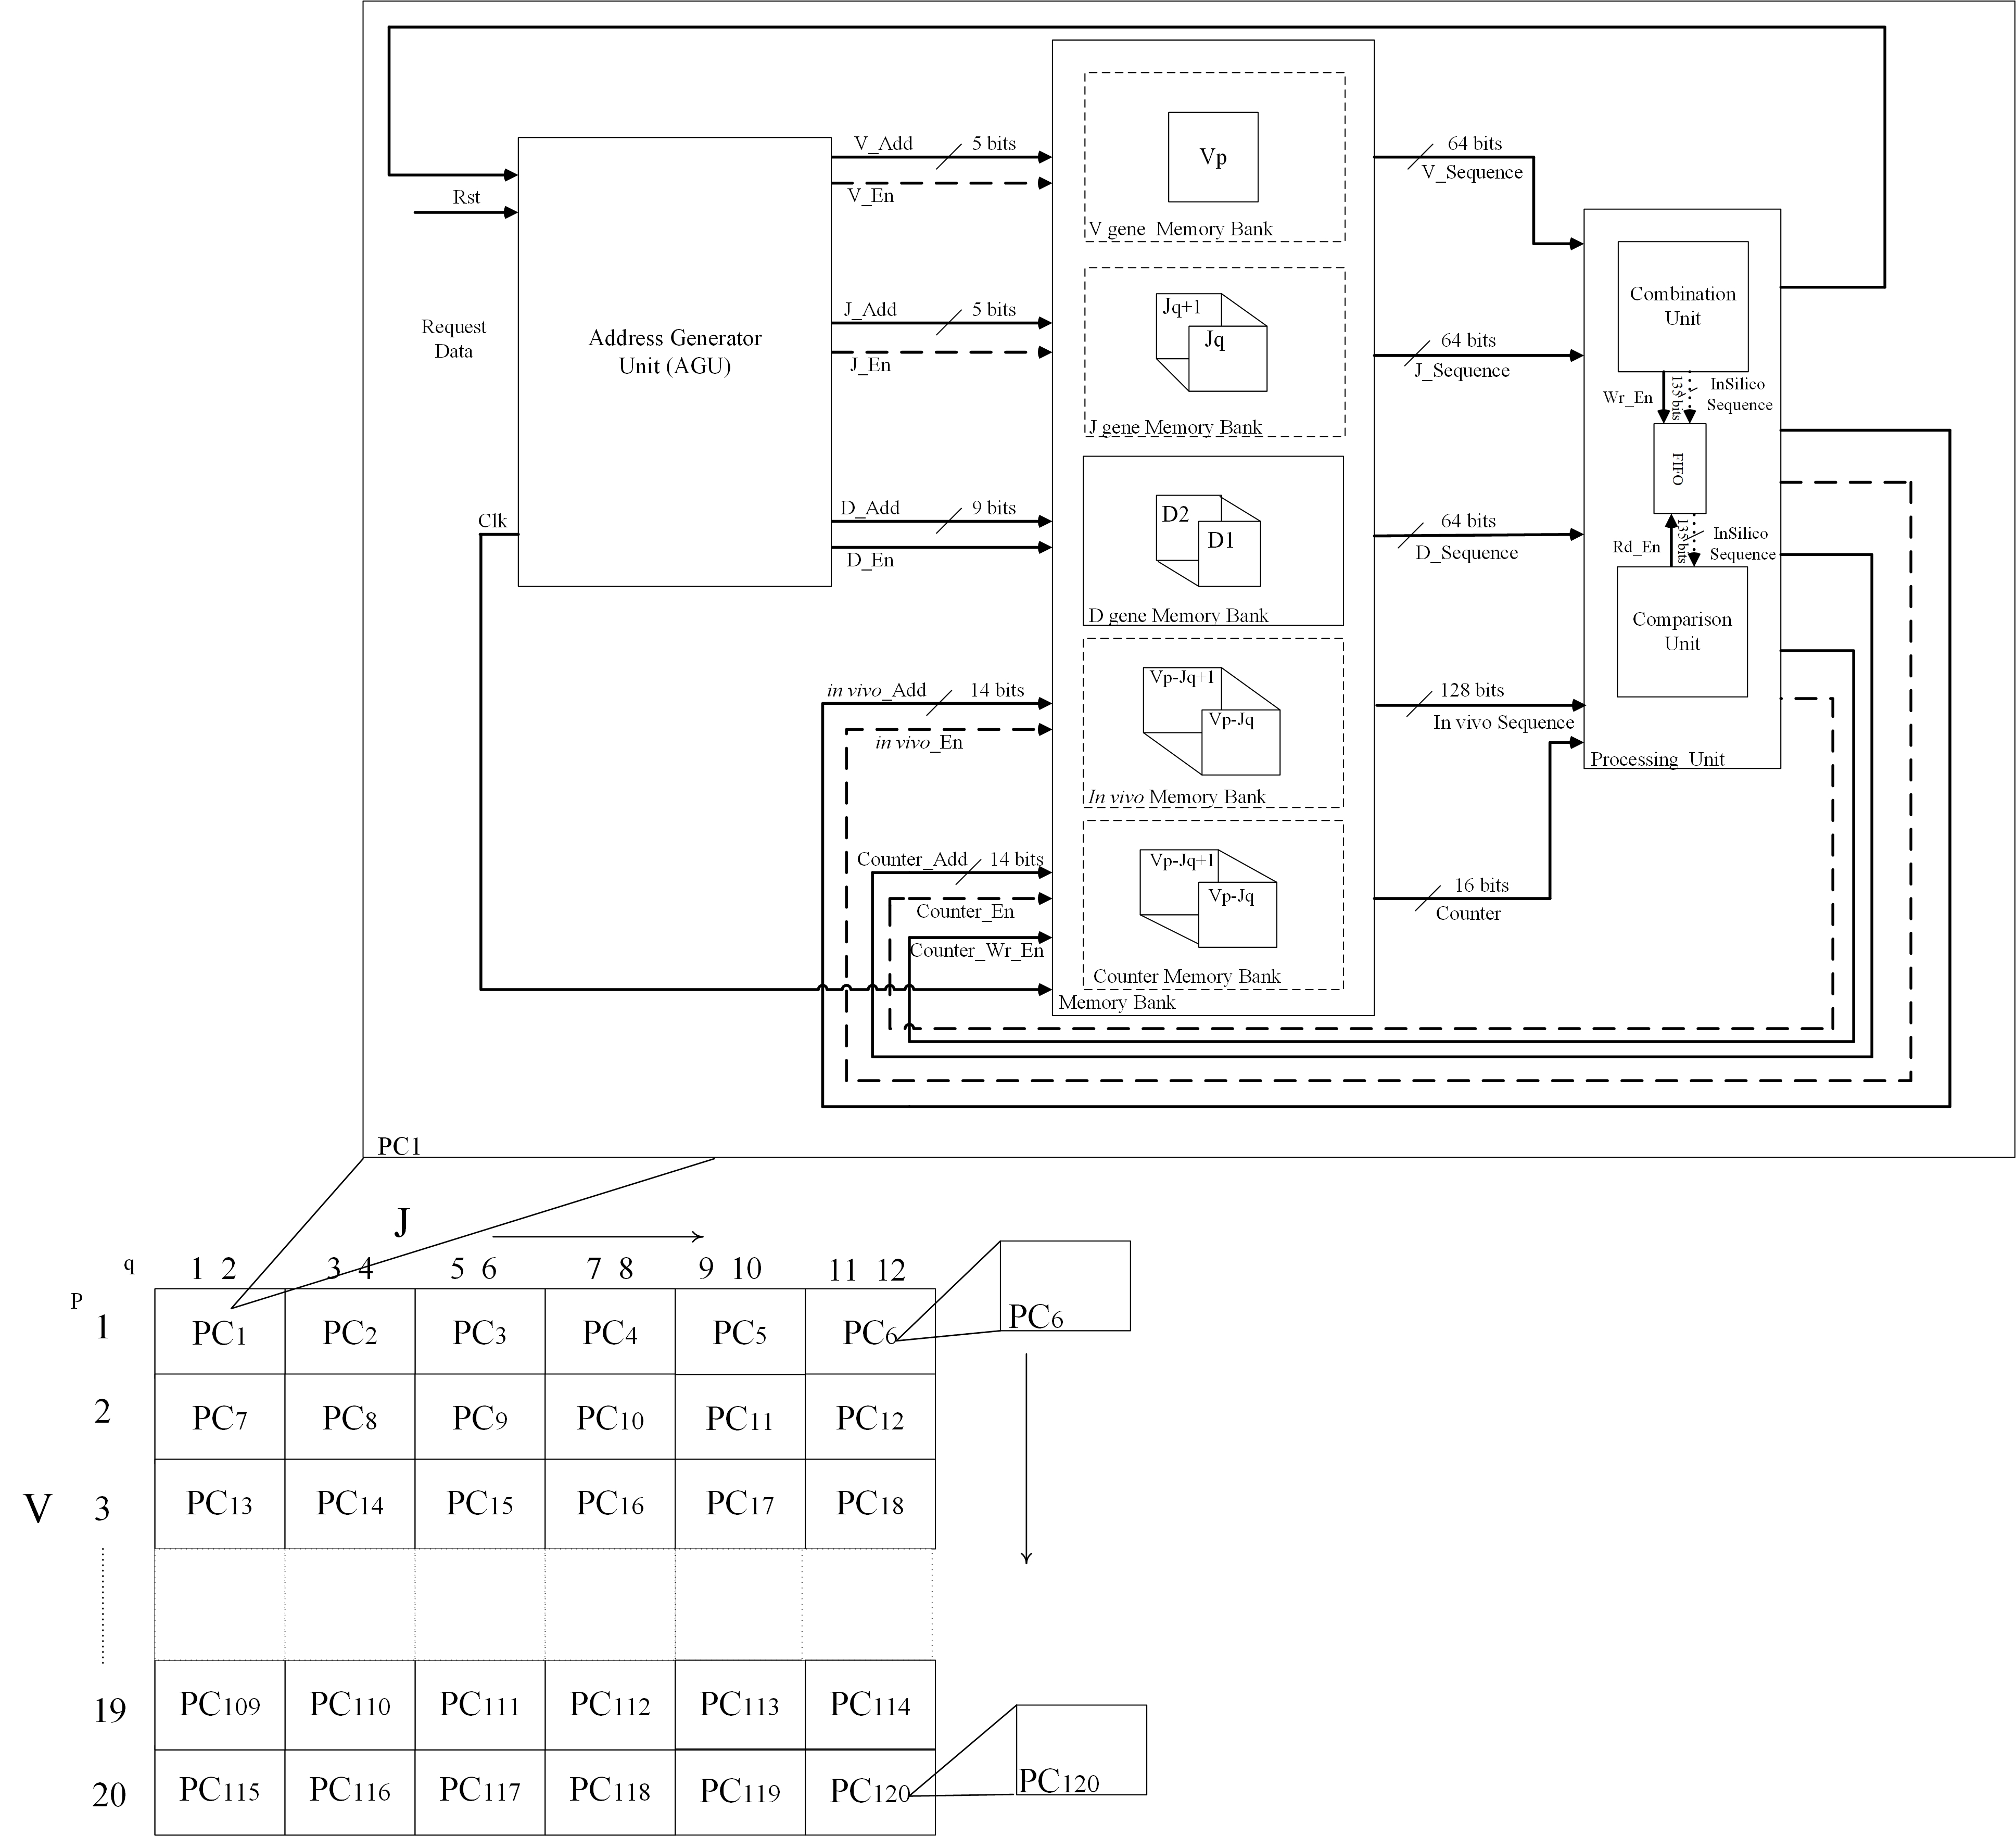
\includegraphics[clip,width=1\columnwidth]{Fig/BIG-Picture_VJLevel.jpg}
\caption{A high level view of hardware implementation of VJ level parallelization for the $V(D)J$ recombination process.}
\label{fig:BIG-Picture_VJLevel}
\end{center}
\end{figure*}


%%%%%%%%%%%%%%%%%%%%%%%%%%%%%%%%%%%%%%%
\subsection{Combination Unit }\label{subsec:Comb}
%%%%%%%%%%%%%%%%%%%%%%%%%%%%%%%%%%%%%%
The inputs to the combination unit are the $V$, $J$ and $D$ gene sequences received from their respective memory banks. The addresses for these three sequences are determined by the AGU, which will be discussed later. We set the bitwidth for each sequence to 64 bits as shown in Fig. \ref{fig:BIG-Picture_VJLevel}.  In C57BL/6 mice data set, the maximum length of the  $V$, $J$ and $D$ gene sequences is 26 characters. We assign two bits to represent each of the four types of nucleotide bases (A, G, C, and T). We reserve six bits to keep track of the length of each sequence. The combination unit will rely on this length information for the \emph{in silico} generation.  As explained earlier in section \ref{sec:DNA}, the $D$ gene goes through chewback process on its both ends. Based on the C57BL/6 mice data set,  there are maximum of 22 different paths to generate $D$ sequences. We reserve five bits to represent each path, which we refer to as $D_{Path}$. The comparison unit will require this information for counter update, which will be discussed later. Therefore, in total we need form a 63 bit package as in input to the Combination Unit, however we set the package size as 64 leaving 1-bit  for debugging purpose to set as used or not used. The combination unit continuously executes the following five steps as long as the buffer is not full to implement the for loops indexed four and five of the Algorithm \ref{Algorithm:2}. Fig. \ref{fig:CombinationUnit} shows the high level flow of these five steps.
 
\emph{Step 1:} We set the length of n-nucleotide to zero as a starting point. For the current 64-bit  $V$, $J$ and $D$, we extract the length of each sequence and calculate the length of \emph{in silico} sequence using (\ref{eq:4}). Based on the C57BL/6 mice data set there are two conditions that need to be met in terms of the \emph{in silico} sequence length. Length of the generated sequence must be within the range of six to sixty characters and divisible by three. If the length of \emph{in silico} sequence meets those two conditions, then we set the initial binary value of the n-nucleotide sequence as zero for the current n-nucleotide length and proceed to the step two. If the length conditions are not met,  then we check the length of n-nucleotide.  If the length of n-nucleotide is less than ten then, we increase the length of n-nucleotide by one, update the length of \emph{in silico} sequence, and  reevaluate the new length. If the length of n-nucleotide is not less than ten then, we request a new input data from the V, D, and J memory banks, whose addresses are generated by the AGU.

\begin{equation}\label{eq:4}	
Length_{\emph{in silico}} = V[5:0] + J[5:0] + D[5:0]+ n-nucleotide_{length}
\end{equation} 
 
\emph{Step 2:} The n-nucleotide sequence involves the $n_1$ and $n_2$ nucleotide sequences \ref{subsec:Bio}. In the second step, we set the length of $n_1$ and $n_2$ sequences based on the length of n-nucleotide, which was selected in the previous step.  We set the length of $n_1$ sequence equal to the length of n-nucleotide and set the length of $n_2$ sequence equal to zero, then we continue on to the third step. Later in step five we will decrement and increment the $n_1$ and $n_2$ lengths by one respectively till $n_1$ is 0 and $n_2$ is the length of n-nucleotide. 

\emph{Step 3:} In this step,  we use an \emph{or} gate to concatenate the $V$, $n_1$  $D$,  $n_2$ and $J$ sequences in the given order to form a 134-bit sequence. The position of each sequence in the 134-bit package is determined by the length of the remaining four sequences. This position value is used as the shift amount to apply to each sequence before the \emph{or} gate based concatenation. As mentioned before, the maximum length of an \emph{in silico} sequence is 60 characters (120 bits). We reserve six bits to keep track of the length of \emph{in silico} sequence ($sequence_{length}$), two bits to keep track of the $VJ$ group $group_{id}$, five bits to indicate the $D_{Path}$, and one bit as a $n_{length}$ flag to show that the \emph{in silico} sequence is created using the n-nucleotide with length of greater than zero. The comparison unit relies on the \emph{in silico} length information and $VJ$ group to reduce its search space, which we will explain later.
%set the \emph{in silico} sequence length to 128 bits.


\emph{Step 4:} In this step, we check the status of the the first-in, first-out buffer (FIFO). If the FIFO is not full, then we pass the generated 134-bit sequence into the buffer and proceed to the fifth step. Otherwise, we remain in this step till the last entry in the buffer becomes available.   

\emph{Step 5:} At this point of the execution, the combination unit has generated an \emph{in silico} sequence and fed it into the FIFO. This step adjusts the lengths of n1 and n2 sequences along with the binary value of the n-sequence based on the following execution model. We first evaluate the length of $n_1$ sequence. If it is greater than zero, then we increase the length of $n_2$ sequence, decrease the length of $n1$ sequences, and proceed to the third step. We increase and decrease the length $n_1$ and $n_2$ respectively to generate all possible combinations of $n_1Dn_2$ sequence. 

When the length of $n_1$ sequence reaches to zero, we compare the current binary value of the n-nucleotide sequence with the largest number that can be generated for that length (note that length was determined in Step 1). If it does not match, then we increase the n-nucleotide value by one and move to the second step. Otherwise, we move to the first step to evaluate and increase the length of n-nucleotide. Indeed, all possible forms of n-nucleotide sequence can be generated by increasing its value by one. Since all zeros in the n-nucleotide sequence is equivalent to the sequence with all 'A', while the n-nucleotide sequence with all ones is equal all 'T'. 
\begin{figure}
\begin{center}
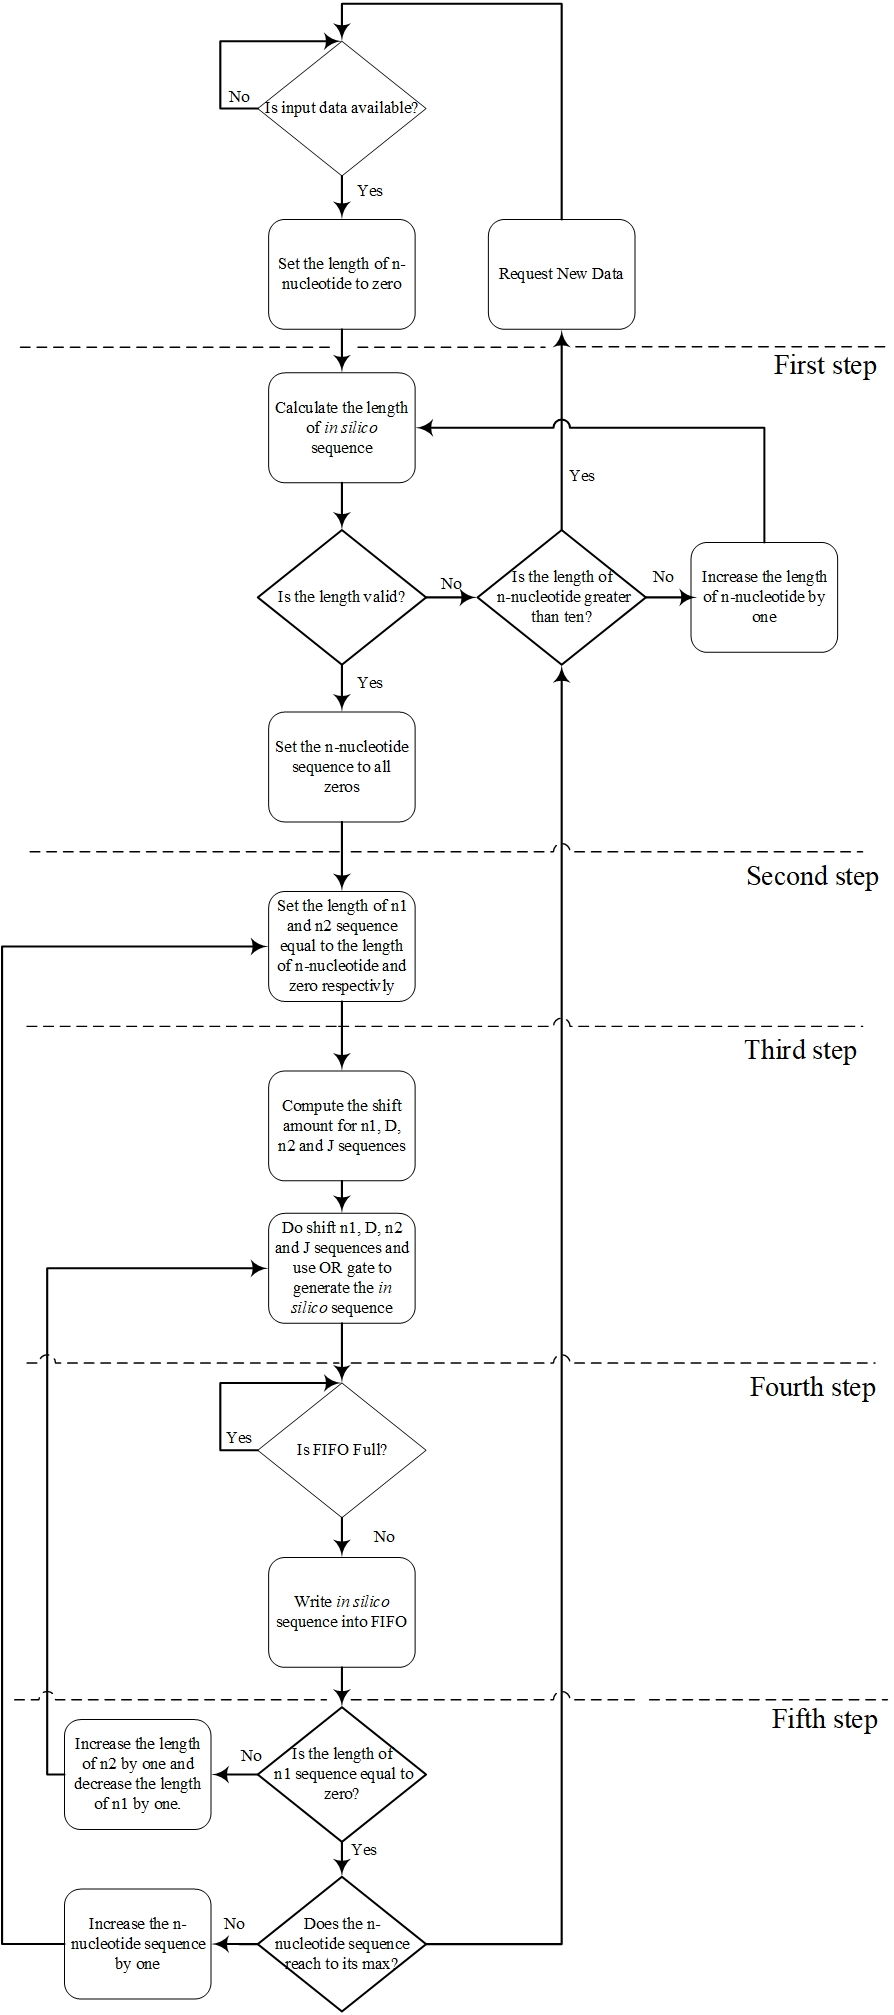
\includegraphics[clip,width=0.6\linewidth]{Fig/Combination_Unit.jpg}
\caption{The algorithmic description for the structure of Combination unit.}
\label{fig:CombinationUnit}
\end{center}
\end{figure}

\subsection{Comparison Unit }\label{subsec:Comp}
%%%%%%%%%%%%%%%%%%%%%%%%%%%%%%%%%%%%%%
The inputs for the comparison unit are 134-bit package received from the buffer, 128-bit \emph{in vivo} sequence received from the \emph{in vivo} memory bank, and the 16-bit counter indicating the number of times that specific \emph{in vivo} sequence has been generated. Before we describe the functionality of the comparison unit, we explain the structure of the \emph{in vivo} memory bank. As mentioned in section \ref{subsec:parallel VJ Level}, we distribute the \emph{in vivo} data set across the PCs based on the $VJ$ group assignment. Since we pair each $V$ gene with two $J$ genes, we divide the \emph{in vivo} memory bank into two partitions, where each partition holds  \emph{in vivo} sequences sorted in ascending order of length for that $VJ$ group. This way of data organization allows us to use the $group_{id}$ to search for the data only in one of the two partitions, and $sequence_{length}$ to search within a single group among the sequences that have the same length. In order to realize this, we need to know the starting and ending addresses of the \emph{in vivo} sequences in the \emph{in vivo} memory bank for any given $sequence_{length}$ and $group_{id}$. Therefore, we utilize two $2$x$19$ arrays ($starting_{array}$, $ending_{array}$), which keep the starting and ending address of \emph{in vivo} sequences for every $sequence_{length}$ and $group_{id}$. The size of $starting_{array}$, $ending_{array}$ is defined based on the total number of $VJ$ group in each PC (two $VJ$ groups) and the total number of available length for the \emph{in vivo} sequence (19 different lengths from six to sixty characters).

The comparison unit continuously executes the following four steps as long as there is data in the buffer to implement the inner most for loop of the Algorithm \ref{Algorithm:2}. Fig. \ref{fig:ComparisonUnit} shows the high level flow of these four steps.

\emph{Step 1:} In this step, we check whether the buffer has at least four entries or not.  We remain in this step till the combination unit passes at least four \emph{in silico} sequences to the buffer.

As mentioned before, there are four nucleotide bases (A, C, G, and T) that we need to use for generating the n-nucleotide sequences. Therefore, there are $4^M$ n-nucleotide sequences with length of $M$ involving in the recombination process. In addition, we need to generate all possible combinations of $n_1Dn_2$ in the recombination process (step five of the combination unit) for any given n-nucleotide sequence in the presence of $D$ sequence ($D$ sequence with length of greater than zero). This causes additional $M+1$ ways for generating the \emph{in silico} sequence for a given n-nucleotide. Therefore, the total number of possible \emph{in silico} sequences for a given $V$, $D$, and $J$ genes is equal to $4^M \times $($M+1$) using the n-nucleotide sequence with length of $M$. Based on this analysis, we have at least $4^M \times $($M+1$) \emph{in silico} sequences with the same features ($sequence_{lenght}$, $group_{id}$, and $D_{path}$) in the presence of n-nucleotide and $D$ sequence. However, we have at least $4^M$ \emph{in silico} sequences with the same features in the absence of $D$ gene. Table \ref{tab:2} shows the total number of \emph{in silico} sequences with the same features for a given n-nucleotide with length of $M$ in the presence and absence of $D$ sequence. 

We can benefit from the above feature to perform parallel comparisons to accelerate the process. However, the level of parallelization is dependent on the length of n-nucleotide and $D$ gene in the recombination process. The parallelization level affects the resource utilization and execution time performance. Increasing the parallelization level results in increasing the resource utilization directly as we need to provide a 134-bit register for every \emph{in silico} sequences in the comparison unit. The execution time reduces as we increase the parallelization level from one to two/four. However, increasing the parallelization level from four to eight increases the critical path delay due to higher resource utilization. Also, this solution is not applicable for all the cases as shown in the table \ref{tab:2}. Therefore, we set the parallelization level to four to have a general solution for most of the cases and avoid increasing the resource utilization. Note that we can not do any parallelization in the absence of n-nucleotide (length of n-nucleotide equal to zero). Thus, we detect this case at the second step using the $n_{length}$ flag to perform the comparison process without parallelization. 

\begin{table}[t!]
\caption{The total number of \emph{in silico} sequences with the same features for a given n-nucleotide's length with and without the $D$ gene.}
\begin{center}
\begin{tabular}{ |c|c|c| }
  \hline
    $N_{Length}$ & \textbf{\textit{Total number of sequences }}& \textbf{\textit{ Total number of sequences}} \\	
    ~ & \textbf{\textit{in the presence of  $D$ gene}} & \textbf{\textit{in the absence of $D$ gene}} \\		\hline
    0 & 1 & 1 \\	\hline
    1 & 8 & 4\\	\hline
   	2 & 48 & 16 \\	\hline
    3 & 256 & 64\\	\hline
    4 & 1280 & 256 \\	\hline
    5 & 6144 & 1024 \\	\hline
    6 & 28672 & 4096\\	\hline
   	7 & 131072 & 16384 \\	\hline
    8 & 589824 & 65536\\	\hline
    9 & 2621440 & 262144 \\	\hline
    10 & 11534336 & 1048576\\
  \hline
\end{tabular}

  \label{tab:2}
\end{center}
\end{table}  

\emph{Step 2:} In this step, we first read one \emph{in silico} sequence from the buffer. If the $n_{length}$ of the received sequence is set to one, then we read three more \emph{in silico} sequences from the buffer and proceed to the third step. Otherwise, we directly continue on to the third step. 
%Note that the information related to the length of n-nucleotide is placed into the 134-bits package in the fourth step of combination process. 

\emph{Step 3:} At this step, there is no difference between having one or four \emph{in silico} sequences since all of them have the same features. Therefore, we first extract the $sequence_{lenght}$ and $group_{id}$ of the \emph{in silico} sequence. Then, we calculate the index of $starting_{array}$ and $ending_{array}$ based on $group_{id}$ and $sequence_{lenght}$ using (\ref{eq:5}). Accordingly, we can access to the starting address and ending address of \emph{in vivo} memory using the calculated index. Finally, we set the address of \emph{in vivo} memory bank to the starting address and proceed to the next step.

\begin{equation}\label{eq:5}	
Index_{array} = group_{id} \times 19 + \frac{sequence_{length}} {2} - 2
\end{equation} 

\emph{Step 4:} In this step, we first read the \emph{in vivo} sequence from the \emph{in vivo} memory bank. Then, we compare the  \emph{in vivo} sequence with  \emph{in silico} sequences  simultaneously. If there is a match between the \emph{in silico} and \emph{in vivo} sequences, then we set the address of counter memory bank to the current address of \emph{in vivo} and proceed to the next step. Otherwise, we compare the current address of \emph{in vivo} memory bank with the ending address of \emph{in vivo} memory bank that is determined in the previous step. If it is match, then we go to the first step. Otherwise, we increment the current address  of \emph{in vivo} memory bank by one, read the next \emph{in vivo} sequence, and do comparison.

\emph{Step 5:} In this step, we first read the \emph{counter} from the counter memory bank. Then, we update the \emph{counter} value with the $D_{path}$ and write the updated \emph{counter}  into the counter memory bank. At this point, if we find a match for all of the \emph{in silico} sequences,  then we move to the first step. Otherwise we continue on to the fourth step to do the comparison between the current address of \emph{in vivo} memory bank and the ending address.

\begin{figure}
\begin{center}
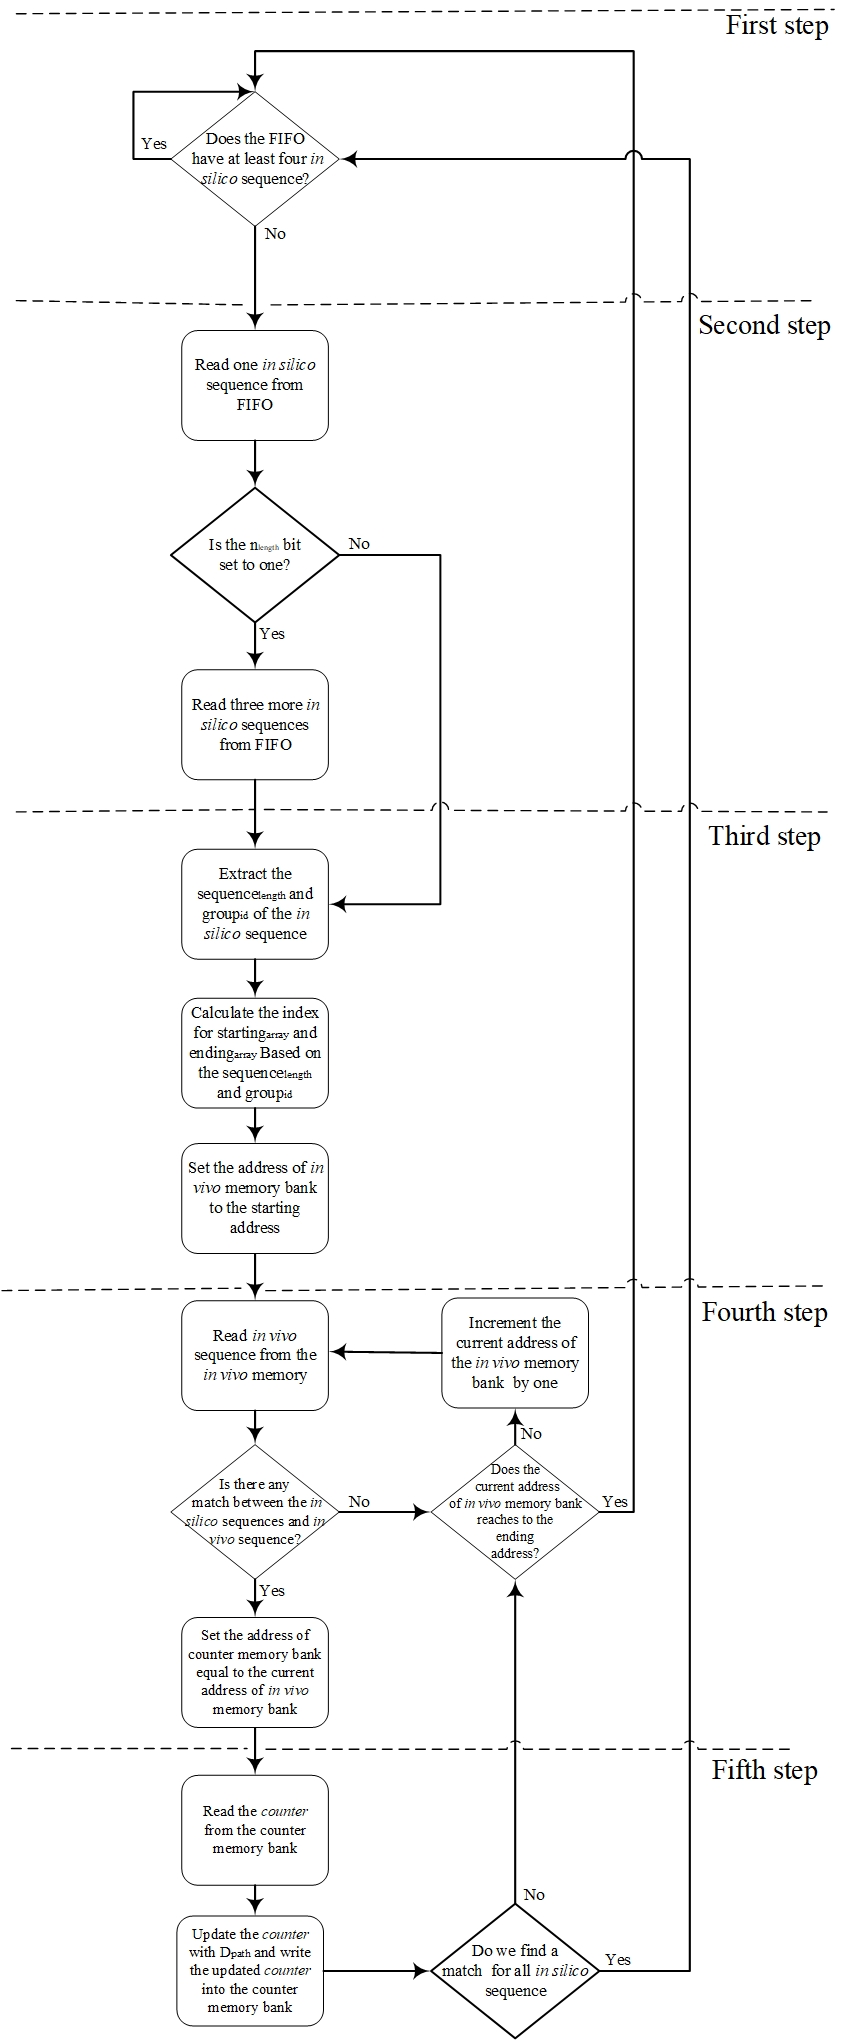
\includegraphics[clip,width=0.6\linewidth]{Fig/Comparison_Unit.jpg}
\caption{The algorithmic description for the structure of Comparison unit.}
\label{fig:ComparisonUnit}
\end{center}
\end{figure}
\subsection{First In First Out Buffer (FIFO)} \label{subsec:FIFO}
%%%%%%%%%%%%%%%%%%%%%%%%%%%%%%%%%%%%%%
We utilize FIFO in the PUs for three reasons. First, we can eliminate the communication overhead between the combination and comparison units, since the combination unit continuously generates the \emph{in silico} sequence and passes it to the FIFO without considering the state of comparison unit. Also, the comparison unit can perform comparison as long as the buffer is not empty without considering the state of combination unit. 
Second, we can perform parallel comparisons using FIFO. Third, we can overlap the task of combination and comparison units using the FIFO, which results in reducing the execution time.
The challenging decision for the FIFO relates to its size. The size of FIFO directly affects the BRAM utilization. We use $75\%$ of the available BRAM in the target FPGA without the FIFO. Since our aim is to remain below $85\%$ BRAM utilization, we can only assign $1 \times 36Kb$ BRAM to each PU. Thus, we set the FIFO so that it can keep up to 256 \emph{in silico} sequences with 134 bits.   


\section{Simulation Results of the VJ Level Parallelization Architecture} \label{sec:simVJlevel}

Table \ref{tab:7} shows the resource utilization for the VJ level parallelization architecture. As shown, we utilize up to the 80\% of the available resources on the target FPGA. The critical path delay is 9.328  $ns$ and the maximum clock rate is 100 MHz. Table \ref{tab:4} shows the execution time for each $N_{Length}$ for both n-level and VJ level parallelization approaches on Virtex-7 FPGA along with the execution time for the baseline GPU-based implementation on K20 GPU. The total execution time for the VJ level parallelization approach is equal to 8237 minutes (($\sim$ 5.7 days)) on the target FPGA. As stated in table \ref{tab:6}, the total execution time for the VJ level approach reduces by a factor of 2.37 in comparison with the n-level parallelization approach. In addition, the execution time for n-nucleotide length of zero to seven on FPGA is smaller than the GPU-based implementation. However, for the large length of n-nucletide, the execution time for GPU-based implementation is faster by a factor of 1.2. As a result the total execution time for the VJ level parallelization approach is slower than the baseline GPU-based implementation by a factor of 1.13.   

\begin{table}[t!]
\caption{Execution time for the n-level and VJ level parallelization approach for FPGA-based implementation using Virtex-7 in comparison with the state-of-the-art GPU-based implementations using K20.}
\begin{center}
\scalebox{0.7}{
\begin{tabular}{ |c|c|c|c|}
  \hline
   $N_{Length}$ & \textbf{\textit{Execution time (min)}}& \textbf{\textit{Execution time (min) }}& \textbf{\textit{Execution time (min)  }}  \\	
   ~ & \textbf{\textit{  for n-level parallelization }} &\textbf{\textit{for VJ level parallelization}}& \textbf{\textit{for the state-of-the-art}}\\
   ~& \textbf{\textit{approach using Virtex-7}} &\textbf{\textit{ approach using Virtex-7}} & \textbf{\textit{ GPU-based implementation }}\\ 
   ~ &~&~&\textbf{\textit{using K20 GPU}}\\ \hline
	0	& \textless 1	& \textless 1 	& 27  \\	\hline	
	1	&1	&\textless 1 	& 32  \\	\hline	
	2	&1	&\textless 1 	& 39 \\	\hline	
	3	&1	&\textless 1 	& 46 \\	\hline	
	4	&1	&\textless 1 	& 55 \\	\hline	
	5	&8	&3   & 64 \\	\hline	
	6	&39 &17  &67     \\	\hline
	7	&180&78  &83    \\	\hline
	8	&805&347 &331    \\	\hline
	9	&1768&1490 & 1290   \\	\hline
	10	& 15243  & 6300& 5261 \\ \hline  	
   	Total &19571 & 8237 & 7295\\	
  \hline
\end{tabular}}

  \label{tab:6}
\end{center}
\end{table}
\begin{sidewaystable}
    \centering
%\begin{table}[t!]
\caption{FPGA Resource Utilization for the VJ Level Parallelization Architecture.}
\scalebox{0.7}{
\begin{tabular}{ |c|c|c|c|c|c|c|c| }
  \hline
    \textbf{\textit{Component}} & \textbf{\textit{Slice LUTs}} & \textbf{\textit{Slice Registers}}  & \textbf{\textit{Slice}}  & \textbf{\textit{F7 Muxes}}  &  \textbf{\textit{F8 Muxes}} & \textbf{\textit{LUT Flip Flop Pairs}}  & \textbf{\textit{BRAM}}  \\	
    ~ & \textbf{\textit{303600}} & \textbf{\textit{607200}} & \textbf{\textit{75900}} & \textbf{\textit{151800}} & \textbf{\textit{75900}} & \textbf{\textit{303600}} & \textbf{\textit{1030}} \\	\hline
	Combination unit & 127080 & 22440 & 38400 & 0 &  0 & 13200 & 0 \\	\hline   
	Comparison unit & 93000 & 62520 & 30000 & 120  &  0 & 61440& 0\\	\hline
	FIFO & 3840 & 4680 & 2040 & 0 &  0 & 2520 & 240 \\	\hline 
	AGU & 4440 & 2880 & 1560 & 0 &  0 & 2880 & 0 \\	\hline    
    $V$ memory bank unit & 840 & 0 & 360 & 0 &  0 & 0& 0 \\	\hline
   	$J$ memory bank unit & 4800 & 0 & 3720 & 0 &  0 &0& 0 \\	\hline
   	$D$ memory bank unit & 15000 & 0 & 4200 & 2880 &  1440 & 0& 0\\	\hline
   	$in~vivo$ memory bank unit & 0 & 0 & 0 & 0 &  0 &0& 452 \\	\hline
   	$counter$ memory bank unit & 0 & 0 & 0 & 0 &  0 & 0&70 \\	\hline
   	glue and display logics & 1431 & 216 & 469 & 4 &  0 & 98&0 \\	\hline
   	Total & 245991 &  92736& 68385 & 3004 & 2880& 80040 & 762  \\	\hline
   	Percent & 81\% & 15\% & 90\% & 1.9\% & 3.7\% & 26\% & 73.9\% \\
   	
  \hline
\end{tabular}
}
  \label{tab:7}

%\end{table}
\end{sidewaystable}
